\subsubsection{CFD-DEM}

\noindent
\justify

El acoplamiento entre CFD \textit{(``Computational Fluid Dynamics")} y DEM \textit{(``Discrete Element Method")} busca predecir la interacci\'on fluido-part\'icula. El flujo se resuelve a trav\'es de CFD basado en malla (ver secci\'on \ref{CFD:problema}), mientras que la fase s\'olida es modelada mediante DEM para cada part\'icula sujeta a trav\'es de fuerzas hidrodin\'amicas, fuerzas de cuerpo (como la gravedad) y a trav\'es de fuerzas de contacto; actualizando valores de velocidad y posici\'on conforme a la segunda ley de Newton (Hoomans \textit{et al.}, 1996; Tsuji \textit{et al.}, 1993; Xu y Yu, 1997). 

\noindent
\justify

La tasa de part\'iculas debido a la sedimentaci\'on, a trav\'es de canales inclinados, ha sido ampliamente estudiado debido al reconocido \textit{efecto Boycott}$^{\cite{Xu2005}}$. Este fen\'omeno se produce por el incremento en el \'area efectiva de sedimentaci\'on debido a la presencia de placas inclinadas$^{\cite{Galvin2002}}$. Acrivos \textit{et al.} han desarrollado una serie de planteamientos te\'oricos y experimentales entre la tasa de sedimentaci\'on de part\'iculas y el \'area efectiva de sedimentaci\'on. El efecto Boycott ha sido aplicado con \'exito en diversos procesos industriales para la remoci\'on de part\'iculas en lecho de fluidizado a trav\'es del asentamiento gravitacional; entre los principales ejemplos de este hecho se encuentran: tratamientos de aguas residuales y procesos de filtrado de agua.

\noindent
\justify

El acercamiento experimental para la investigaci\'on caracter\'istica de part\'iculas en suspenci\'on a alta concentraci\'on ha demostrado ser una experiencia retadora debido a las limitantes instrumentales y t\'ecnicas de medici\'on$^{\cite{Galvin2002}}$. Los modelos num\'ericos basados en CFD han demostrado ser una herramienta poderosa y promisoria que provee informaci\'on detallada y precisa sobre las caracter\'isticas locales del flujo particulado. Normalmente, se han aplicado dos enfoques generales en la literatura para resolver problemas que involucran flujo particulado: \textit{Eulerian - Eulerian} (E-E) y \textit{Eulerian - Lagrange} (E-L). En el enfoque E-E, las fases s\'olida y fluida son interpretadas de manera continua en donde comparten el mismo grupo de ecuaciones gobernantes. Doroodchi \textit{et al.}$^{\cite{Doroodchi2005}}$ emplearon el modelo E-E para investigar la influencia de las placas inclinadas y el efecto expansivo de s\'olidos en suspensi\'on en camas de lecho fluidizado; obteniendo resultados prometedores tanto en la parte experimental como num\'erica. Salem \textit{et al} $^{\cite{Salem2011}}$ desarrollaron un modelamiento en CFD empleando el modelo E-E para evaluar las caracter\'isticas hidr\'aulicas de un sedimentador de placas hidr\'aulicas (IPS, por sus siglas en ingl\'es); demostrando el importante rol que cumplen las herramientas computacionales en el estudio de los sistemas de sedimentaci\'on. Sin embargo, el tratamiento de la fase s\'olida de manera continua va en contra de la naturaleza discreta de las part\'iculas s\'olidas, y todav\'ia m\'as importante: el acercamiento a trav\'es de E-E carece de facultades num\'ericas para revelar informaci\'on importante referente a la escala particular.

\noindent
\justify

El enfoque otorgado por el modelo E-L, por otro lado, adopta la teor\'ia continua para la fase l\'iquida y resuelve el problema cinem\'atico de cada part\'icula individual \textbf{directamente}. Informaci\'on referente a la posici\'on, velocidad, fuerza hidrodin\'amica y difusividad, entre otros, se pueden obtener para cualquier instante de tiempo. Teniendo as\'i el potencial de sobrellevar las dificultades y limitaciones existentes en modelos te\'oricos y emp\'iricos. Es debido a ello que en el \textit{presente trabajo} se emplea un enfoque E-L para abordar el problema CFD-DEM; investigando la interacci\'on fluido - part\'icula en un sistema de sedimentaci\'on con canales (lamelas) inclinadas.

\paragraph{Planteamiento num\'erico}

\noindent
\justify

El flujo del modelo CFD-DEM se resuelve a trav\'es de las ecuaciones de momento, continuidad y a trav\'es de las ecuaciones de movimiento de cada part\'icula individual, seguidas a trav\'es del m\'etodo de elementos discretos$^{\cite{Peng2014}}$. Se consideraron los efectos e interacciones entre part\'icula-part\'icula (ver Figura \ref{particula}), part\'icula-fluido y part\'icula-muro. Las ecuaciones gobernantes y la metodolog\'ia num\'erica empleada se describe brevemente a continuaci\'on.

\begin{figure}[h!]
	\centering
	\begin{subfigure}[b]{0.4\textwidth}
		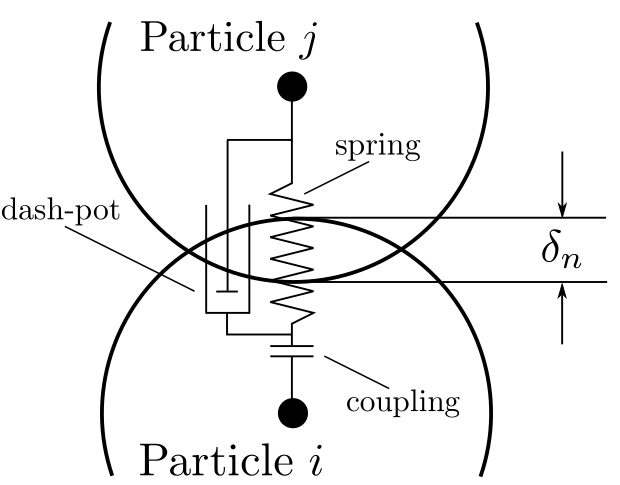
\includegraphics[width=\textwidth]{Images/normal.png}
		\caption{Fuerza normal.}
	\end{subfigure}
	\hfill
	\begin{subfigure}[b]{0.4\textwidth}
		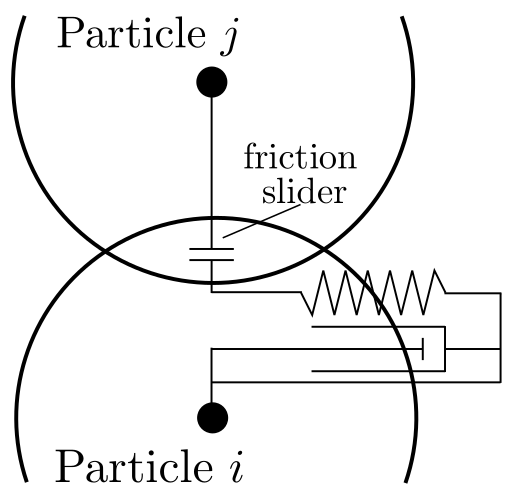
\includegraphics[width=0.8\textwidth]{Images/tangencial.png}
		\caption{Fuerza tangencial.}
	\end{subfigure}
	\caption{Interacci\'on din\'amica entre part\'iculas.}
	\label{particula}
\end{figure}

\noindent
\justify

En DEM, no se requiere de un \textit{cierre} para la fase s\'olida dado que la din\'amica de la part\'icula se resuelve de manera directa. La traslaci\'on y rotaci\'on de la part\'icula $i$ est\'a dada por las Ecuaciones \ref{DEMdyn} y \ref{DEMrot}.

\begin{equation}
	m_i \frac{d v _i}{dt} = F_{c,i} + F_{f,i} + F_{g,i}
	\label{DEMdyn}
\end{equation}

\begin{equation}
	I_i \frac{d \omega _i}{dt} = T_{c,i} + T_{r,i}
	\label{DEMrot}
\end{equation}

\noindent
\justify

Las fuerzas de impacto $\left( F_{c,i} \right)$ y el torque de contacto $\left( T_{c,i} \right)$ fueron calculados por el modelo lineal resorte-dashpot en el que se tuvo en cuenta el efecto hister\'etico causado por el historial de contacto de la part\'icula. La resistencia a la rodadura se calcul\'o empleando la Ecuaci\'on \ref{rolling}.

\begin{equation}
	T_{r,i} = - \sum _{j=0} ^{N_{pc}} \mu _{rol}  \left|F_{cn, ij} \right| \frac{\omega _{ij}}{\left| \omega _{ij} \right|} r_i
	\label{rolling}
\end{equation}

\noindent
\justify

D\'onde $\omega _{ij}$ es la velocidad angular relativa entre las part\'iculas $i$ y $j$; y est\'a definida a trav\'es de la Ecuaci\'on \ref{omega}.

\begin{equation}
	\omega _{ij} = \frac{\omega _i r_i + \omega _j r_j}{r_i + r_j}
	\label{omega}
\end{equation}

\noindent
\justify

La fuerza total actuante del fluido $F_{f,i}$ causada por la distorsi\'on de las l\'ineas de corriente alrededor de la part\'icula, que a su vez produce variaci\'on en el tensor de esfuerzos del fluido, se calcula mediante la Ecuaci\'on \ref{ffi}.

\begin{equation}
	F_{f,i} = - V_i \nabla p + V_i \left( \nabla \cdot \tau _f \right) + \epsilon F_{d,i}
	\label{ffi}
\end{equation}

\noindent
\justify

D\'onde $\tau _f$ es el tensor de esfuerzos viscoso del fluido; que se calcula de la siguiente manera:

\begin{equation}
	\tau _f = \mu _L \left[ \left( \nabla u_L \right) + \left( \nabla u_L \right) ^{-1} \right] + \left(\lambda - \frac{2}{3} \mu \right) \left( \nabla \cdot u_L \right) \overline{I}
\end{equation}

\noindent
\justify

La fuerza de arrastre $F_{d,i}$ del fluido, de la Ecuaci\'on \ref{ffi}, se resuelve a una escala longitudinal mayor que el tama\~no de la part\'icula y est\'a dada por la siguiente relaci\'on matem\'atica:

\begin{equation}
	F_{d,i} = \frac{V_i}{1 - \epsilon} \beta \left( u_L - v_i \right)
\end{equation}

\paragraph{Resultados} \label{CFDEM:resultados}

\noindent
\justify

Para la definici\'on de la interacci\'on part\'icula-part\'icula, fluido-part\'icula y part\'icula-muro se emplearon los datos contenidos en el Cuadro \ref{CFDEMdata}.

\begin{table}[h!]
	\centering
	\begin{adjustbox}{max width = 0.45\textwidth}
	\begin{tabular}{|c|c|}
		\hline
		\textbf{Par\'ametro} & \textbf{Valor} \\ \hline
		\multicolumn{2}{|c|}{\textbf{\textit{Generales}}} \\ \hline
		Material & Arena de r\'io \\ \hline
		Tama\~no de part\'icula $[\mu m]$ & 250 \\ \hline
		M\'odulo de Young & $10 ^6$ \\ \hline
		 N\'umero de part\'iculas por segundo & $22300$ \\
		  \hline
		 Velocidad inicial $[m / s]$ & $0.0097$ \\ \hline
		 $\rho [kg/m^3]$ & 1600 \\ \hline
		 $\nu$ & $0.2$ \\ \hline
		 \multicolumn{2}{|c|}{\textbf{\textit{Coeficientes de par de resorte Dashpot}}} \\ \hline
		 $\alpha$ & $0.12$ \\ \hline
		 $\mu$ & $0.52$ \\ \hline
		 Pasos de resoluci\'on de colisi\'on & 12 \\ \hline
	\end{tabular}
	\end{adjustbox}
	\caption{Datos generales para el desarrollo de la simulaci\'on CFD-DEM.}
	\label{CFDEMdata}
\end{table}

\vspace{-0.8cm}

\noindent
\justify

La simulaci\'on num\'erica desarrollada permiti\'o obeservar el comportamiento din\'amico entre las part\'iculas y el solvente; desarroll\'andose el fen\'omeno de sedimentaci\'on desde la entrada de material debido a la baja velocidad de flujo. El diagrama de contorno de velocidades del sistema se puede apreciar en la Figura \ref{CFDEM:vel}.

\begin{figure}[h!]
	\centering
	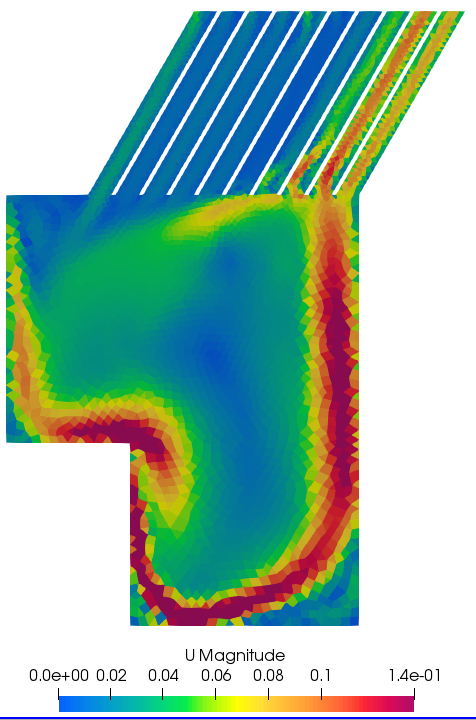
\includegraphics[width=0.31\textwidth]{Images/CFDEM/vel.png}
	\caption{Diagrama de contorno de velocidades del sistema.}
	\label{CFDEM:vel}
\end{figure}

\newpage

\noindent
\justify

El diagrama de contorno de presiones del sistema de sedimentaci\'on se puede apreciar en la Figura \ref{CFDEM:p}.

\begin{figure}[h!]
	\centering
	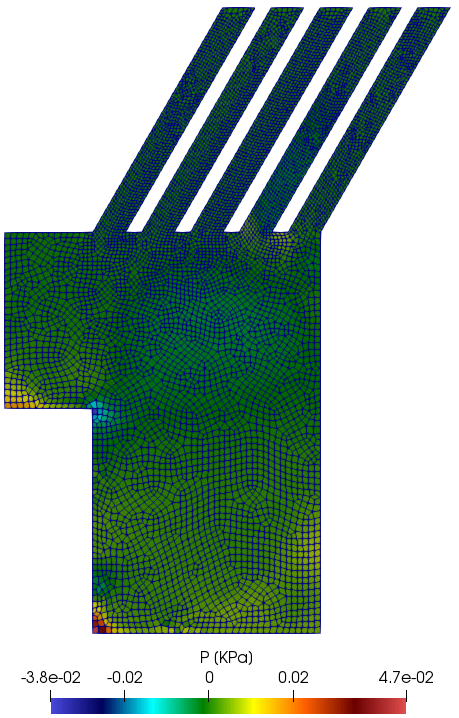
\includegraphics[width=0.31\textwidth]{Images/CFDEM/p.png}
	\caption{Diagrama de contorno de presiones del sistema de separaci\'on de sustancias.}
	\label{CFDEM:p}
\end{figure}

\noindent
\justify

Durante la simulaci\'on, en el que se analizaron $30 [s]$, se apreci\'o el desarrollo de v\'ortices y remolinos debido al reflujo de las part\'iculas, como se aprecia en la Figura \ref{CFDEM:part}.

\begin{figure}[h!]
	\centering
	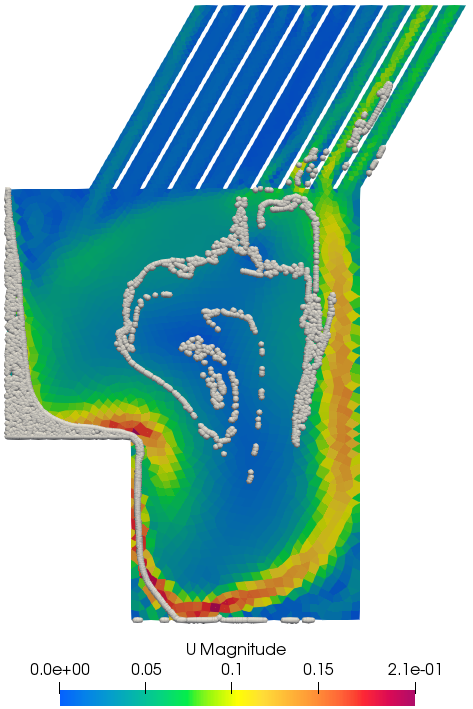
\includegraphics[width=0.355\textwidth]{Images/CFDEM/part.png}
	\caption{Distribuci\'on de part\'iculas de arena sobre el volumen de control durante el segundo $28$ de la simulaci\'on.}
	\label{CFDEM:part}
\end{figure}

\newpage

\paragraph{An\'alisis de resultados} \label{CFDEM:analisis}

\noindent
\justify

Comparando las Figuras \ref{CFD:vel} y \ref{CFDEM:vel}, se puede apreciar c\'omo el solvente cambia la distribuci\'on de velocidades por la sedimentaci\'on sufrida por las part\'iculas de arena, cuya densidad es mayor que la del fluido circundante; raz\'on por la que el solvente tiende a moverse con mayor velocidad en las \'ultimas lamelas en lugar de las primeras, a diferencia de lo observado en la secci\'on \ref{CFD:resultados}. Debido a ello, es posible clasificar a las lamelas por zonas de \textit{``pureza"} durante el proceso de separaci\'on: en donde las primeras seis presentan menor concentrac\'on particular que las \'ultimas cuatro.

\noindent
\justify

La presencia de v\'ortices y remolinos en la simulaci\'on CFD-DEM rectifica la decisi\'on de haber empleado un solucionador basado en \texttt{pimpleFoam}, el cual se adapt\'o para resolver el problema \textit{Euler - Lagrange} (E - L).

\noindent
\justify

Diferente al fen\'omeno apreciado en la Figura \ref{CFD:p}, la distribuci\'on de presiones en la Figura \ref{CFDEM:p} no es sim\'etrica y tiende a presentar sus m\'aximos valores en la zona de congregaci\'on de los sedimentos.

\begin{figure}[h!]
	\centering
	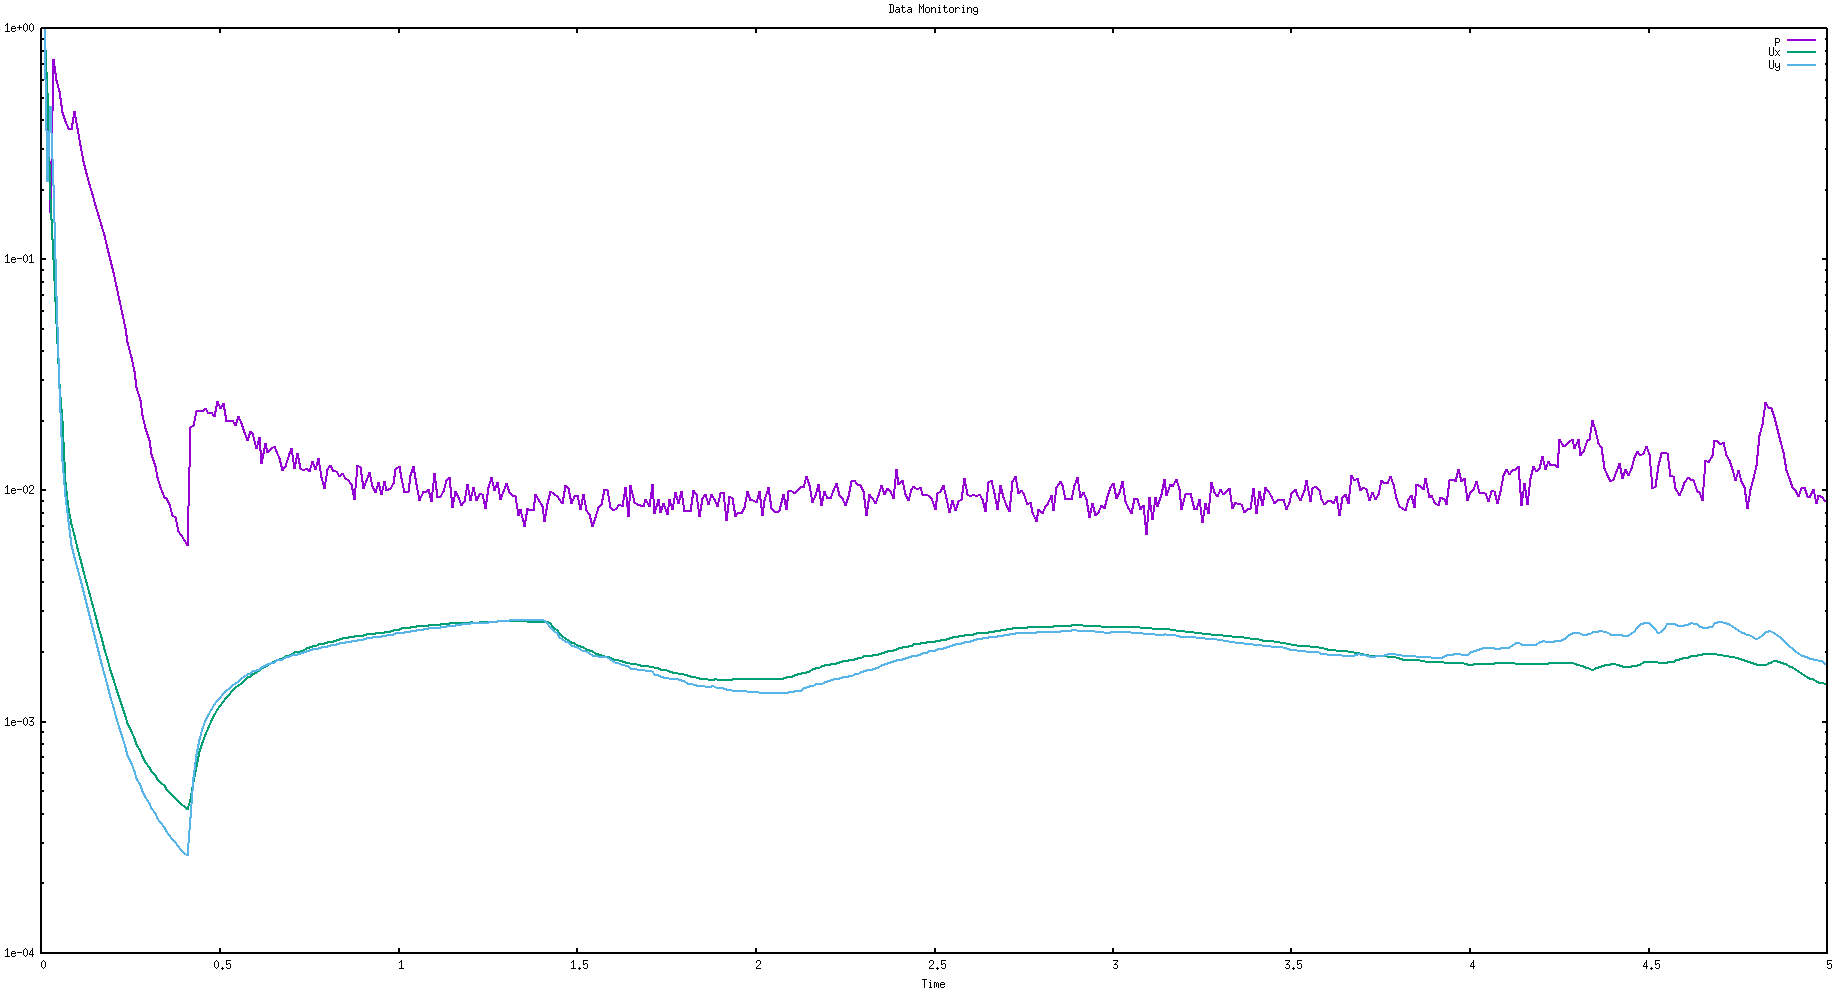
\includegraphics[width=\textwidth]{Images/CFDEM/residuals.png}
	\caption{Monitoreo de residuales en la simulaci\'on CFD-DEM.}
	\label{CFDEM:residuals}
\end{figure}

\noindent
\justify

De la Figura \ref{CFDEM:residuals}, la l\'inea morada corresponde al residual de la presi\'on, la de color cian al residual de la velocidad en $y$ y la de color verde al residual de la velocidad en $x$. El comportamiento de los residuales est\'a directamente relacionado con la magnitud de los errores en la soluci\'on de las ecuaciones gobernantes$^{\cite{Liang2018}}$. Debido al hecho de que tienden a aglomerarse en valores cercanos a cero, son un indicativo de alta precisi\'on del modelo num\'erico implementado. Las variaciones vistas en los residuales de presi\'on se deben a la vorticidad originada por los reflujos consecuentes a la interacci\'on fluido - part\'icula. Durante la simulaci\'on, se observ\'o una estabilizaci\'on en los perfiles de velocidad; raz\'on por la que los residuales $U_x$ y $U_y$ presentan un comportamiento sin fluctuaciones y con peque\~nas variaciones durante el desarrollo del flujo dentro del volumen de control.